\begin{center}
	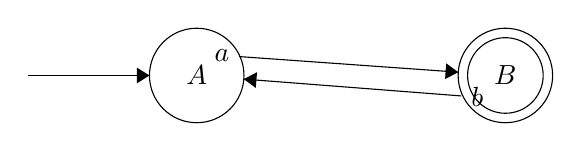
\begin{tikzpicture}[scale=0.2]
		\tikzstyle{every node}+=[inner sep=0pt]
		\draw [black] (12.3,-22) circle (3);
		\draw (12.3,-22) node {$A$};
		\draw [black] (31.9,-22) circle (3);
		\draw (31.9,-22) node {$B$};
		\draw [black] (31.9,-22) circle (2.4);
		\draw [black] (1.6,-22) -- (9.3,-22);
		\fill [black] (9.3,-22) -- (8.5,-21.5) -- (8.5,-22.5);
		\draw [black] (15,-20.8) -- (28.91,-21.79);
		\draw (14.4,-20.76) node [left] {$a$};
		\fill [black] (28.91,-21.79) -- (28.14,-21.23) -- (28.07,-22.23);
		\draw [black] (29.1,-23.3) -- (15.29,-22.23);
		\draw (29.71,-23.35) node [right] {$b$};
		\fill [black] (15.29,-22.23) -- (16.05,-22.79) -- (16.13,-21.79);
	\end{tikzpicture}
\end{center}